% Caution!

% untuk mengedit dokumen, cukup edit file pada bagian :
% /src/chapter
% /src/citation
% /src/image

% jangan edit bagian dibawah ini kecuali anda tahu apa yang anda perbuat.


\documentclass{Proposal_Class}

\usepackage{lipsum}

% info proposal thesis
\def\judulThesis{Judul Thesis Dalam Bahasa Indonesia, Maksimal Jadi Tiga Baris Saja, Kalau Lebih Kecilkan coverSpacing}

\def\tahunPenulisan{2021}
\def\bulanPenulisan{Mei}
\def\tanggalPenulisan{1}

\def\tahunSeminar{2021}
\def\bulanSeminar{Mei}
\def\tanggalSeminar{1}
\def\hariSeminar{Senin}
\def\tempatSeminar{AJ204}

\def\coverSpacing{100mm}


% keterangan prodi dan fakultas
\def\bidangKeahlian{Teknik Sistem Pengaturan}
\def\departemen{Teknik Elektro}
\def\fakultas{Teknologi Elektro}


% keterangan penulis
\def\mahasiswaNama{Nama Lengkap Sekali Mahasiswa}
\def\mahasiswaNRP{NRP Mahasiswa}


% keterangan pembimbing
\def\pembimbingSatuNama{Nama Dosen Pembimbing 1}
\def\pembimbingSatuNIP{NIP. Dosen Pembimbing 1}

\def\pembimbingDuaNama{Nama Dosen Pembimbing 2} % kalau tidak ada, isi dengan {\quad}
\def\pembimbingDuaNIP{NIP. Dosen Pembimbing 2}  % kalau tidak ada, isi dengan {\quad}


% keterangan penguji
\def\pengujiSatuNama{Nama Dosen Penguji 1}
\def\pengujiSatuNIP{NIP. Dosen Penguji 1}

\def\pengujiDuaNama{Nama Dosen Penguji 2}
\def\pengujiDuaNIP{NIP. Dosen Penguji 2}

\def\pengujiTigaNama{Nama Dosen Penguji 3}  
\def\pengujiTigaNIP{NIP. Dosen Penguji 3}   

\def\pengujiEmpatNama{\quad}    % kalau tidak ada, isi dengan {\quad}
\def\pengujiEmpatNIP{\quad}     % kalau tidak ada, isi dengan {\quad}


%% custom command
\def\docContentSpacing{\setlength{\parskip}{.25em}\renewcommand{\baselinestretch}{1.15}}
\def\docDefaultSpacing{\setlength{\parskip}{0em}\renewcommand{\baselinestretch}{1}}

\begin{document}

    \docDefaultSpacing

\begin{titlepage}

    \pagenumbering{roman}
    \setcounter{page}{1}
    
    \thispagestyle{empty}

    % LAMBANG ITS
    \begin{tikzpicture}[overlay,remember picture] 
        \node[anchor=north west, shift={(64mm, 5mm)}] at (current page.north west){
\includegraphics[width=35mm]{src/image/its-lambang.png}}; 
    \end{tikzpicture}
    
    % GARIS KUNING
    \begin{tikzpicture}[overlay,remember picture] 
        \node[anchor=north west, shift={(24mm, -45mm)}] at (current page.north west){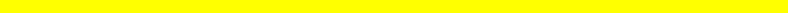
\includegraphics[width=210mm]{src/image/garis-kuning.png}}; 
    \end{tikzpicture}

    % TEKS SAMPUL
    \begin{flushleft}
        \vspace{\coverSpacing}
        \textbf{PROPOSAL THESIS}
    \end{flushleft}

    \vspace{-2mm}\Large
    \begin{flushleft}\textbf{\MakeUppercase{\judulThesis}}\end{flushleft}

    \vspace{10mm}
    \begin{flushleft}
        \normalsize
        \MakeUppercase{\mahasiswaNama} \\
        \MakeUppercase{\mahasiswaNRP} \\
        \vspace{1em}
        DOSEN PEMBIMBING \\
        \pembimbingSatuNama \\
        \pembimbingDuaNama \\
        \vspace{1em}
        PROGRAM MAGISTER \\
        BIDANG KEAHLIAN \MakeUppercase{\bidangKeahlian} \\
        DEPARTEMEN \MakeUppercase{\departemen} \\
        FAKULTAS \MakeUppercase{\fakultas} \\
        INSTITUT TEKNOLOGI SEPULUH NOPEMBER \\
        SURABAYA \\
        \tahunPenulisan
    \end{flushleft}

    
\end{titlepage}

% \restoregeometry{}
    \docDefaultSpacing
\chapter*{LEMBAR PENGESAHAN \\ PROPOSAL THESIS}
\addcontentsline{toc}{chapter}{Lembar Pengesahan}

\begin{center}
    \vspace{5mm}
    \normalsize
    \begin{tabularx}{\textwidth}{l l X*{1}{>{\arraybackslash}X}} 
        Judul   &:  &\judulThesis   \\
        Oleh    &:  &\mahasiswaNama \\
        NRP     &:  &\mahasiswaNRP  \\
    \end{tabularx}

    \vspace{5mm}
    \textbf{Telah diseminarkan pada}

    \vspace{5mm}
    \begin{tabularx}{\textwidth}{l l X*{1}{>{\arraybackslash}X}} 
        Hari    &:  &\hariSeminar                                   \\
        Tanggal &:  &\tanggalSeminar{ }\bulanSeminar{ }\tahunSeminar    \\
        Tempat  &:  &\tempatSeminar                                 \\
    \end{tabularx}

    \vspace{5mm}
    Mengetahui / menyetujui    
\end{center}

\vspace{5mm}
\begin{multicols}{2}
    \begin{flushleft}
        Dosen Penguji: \\

        \vspace{20mm}              
        \pengujiSatuNama\\
        \pengujiSatuNIP\\

        \vspace{20mm}
        \pengujiDuaNama\\
        \pengujiDuaNIP\\

        \vspace{20mm}
        \pengujiTigaNama\\
        \pengujiTigaNIP\\

        \vspace{20mm}
        \pengujiEmpatNama\\
        \pengujiEmpatNIP\\
    \end{flushleft}
    \columnbreak
    \begin{flushleft}
        Dosen Pembimbing: \\

        \vspace{20mm}              
        \pembimbingSatuNama \\
        \pembimbingSatuNIP\\

        \vspace{20mm}
        \pembimbingDuaNama \\
        \pembimbingDuaNIP
    \end{flushleft}
\end{multicols}
    \docContentSpacing

\chapter*{\textbf{\MakeUppercase{\judulThesis}}}
\addcontentsline{toc}{chapter}{Abstrak}


\begin{center}
    \begin{tabularx}{0.75\textwidth}{l l X*{1}{>{\arraybackslash}X}} 
        Nama Mahasiswa  &:  &\mahasiswaNama         \\
        NRP             &:  &\mahasiswaNRP          \\
        Pembimbing      &:  &1. \pembimbingSatuNama \\
                        &   &2. \pembimbingDuaNama 
    \end{tabularx}
\end{center}


\begin{center}
    \large{\textbf{\MakeUppercase{abstrak}}}
\end{center}


%% hapus lipsum dan isi abstrak di sini
\lipsum[1-2]
%% batas pengisian abstrak

\vspace{0mm}
\begin{flushleft}
    Kata kunci: (jumlah kata minimal tiga dan maksimal lima)
\end{flushleft}

    \tableofcontents
    \listoffigures
    \listoftables

    \docContentSpacing

\chapter{Pendahuluan}

\pagenumbering{arabic}
\setcounter{page}{1}

\section{Latar Belakang}{
    % isi section didalam sini
    \lipsum[1-2]
}

\section{Rumusan Masalah}{
    % isi section didalam sini
    \lipsum[3]
}

\section{Tujuan}{
    % isi section didalam sini
    \lipsum[5-6]
}

\section{Batasan Masalah}{
    % isi section didalam sini
    \lipsum[7-8]
}

\section{Kontribusi}{
    % isi section didalam sini
    \lipsum[2]
    \begin{f_itemize}
        \item contoh item satu, boleh panjang boleh pendek. contoh item satu, boleh panjang boleh pendek. contoh item satu, boleh panjang boleh pendek. contoh item satu, boleh panjang boleh pendek.
        \item contoh item satu, boleh panjang boleh pendek. contoh item satu, boleh panjang boleh pendek. contoh item satu, boleh panjang boleh pendek. contoh item satu, boleh panjang boleh pendek.
    \end{f_itemize}
}
    \chapter{Kajian Pusataka}{
    \lipsum[4]
}


\section{Kajian Penelitian Terkait}{
    \lipsum[6]
    \begin{f_enumerate}
        \item contoh item satu, boleh panjang boleh pendek. contoh item satu, boleh panjang boleh pendek. contoh item satu, boleh panjang boleh pendek. contoh item satu, boleh panjang boleh pendek.
        \item contoh item satu, boleh panjang boleh pendek. contoh item satu, boleh panjang boleh pendek. contoh item satu, boleh panjang boleh pendek. contoh item satu, boleh panjang boleh pendek.
        \item contoh item satu, boleh panjang boleh pendek. contoh item satu, boleh panjang boleh pendek. contoh item satu, boleh panjang boleh pendek. contoh item satu, boleh panjang boleh pendek.
    \end{f_enumerate}
    \lipsum[2]
}


\section{Teori Dasar}{
    \lipsum[9-11]
}

\subsection{Cara Membuat Gambar}{
    Untuk menambahkan gambar, simpan gambar dalam folder ./src/image/. Gambar akan diletakkan secara otomatis di tempat yang paling sesuai. cukup tulis perintah latex berikut. setelah itu gambar dapat direferensikan dengan cara menuliskannya seperti \refgbr{fig: lambang its}.
    % SATU GAMBAR DEGAN LABEL 
    \begin{figure}
        \centering
        
\includegraphics[width=.3\textwidth]{src/image/its-lambang.png}
        \caption{Lambang ITS}
        \label{fig: lambang its}
    \end{figure}

    Beberapa gambar dapat ditampilkan secara bersamaan menggunakan subfigure. dan dapat dikutip sebagian, seperti \refgbr{fig:lambang its a}, atau bisa juga hanya diambil penomoran subfigurnya seperti \ref{sub@fig:lambang its b}, atau figurnya secara keseluruhan \refgbr{fig:lambang its semua}.
    \begin{figure}
        \centering
        \begin{subfigure}[b]{0.3\textwidth}
            \centering
            
\includegraphics[width=\textwidth]{src/image/its-lambang.png}
            \caption{Lambang ITS}
            \label{fig:lambang its a}
        \end{subfigure}
        \begin{subfigure}[b]{0.3\textwidth}
            \centering
            
\includegraphics[width=\textwidth]{src/image/its-lambang.png}
            \caption{Lambang ITS juga}
            \label{fig:lambang its b}
        \end{subfigure}
        \begin{subfigure}[b]{0.3\textwidth}
            \centering
            
\includegraphics[width=\textwidth]{src/image/its-lambang.png}
            \caption{Lambang ITS lagi}
            \label{fig:lambang its c}
        \end{subfigure}
        \caption{Lambang-Lambang ITS}
        \label{fig:lambang its semua}
    \end{figure}    
}

\subsection{Cara Membuat Tabel}{
    Di segmen ini akan ditampilkan berbagai macam cara untuk membuat tabel. Untuk membuat tabel kita dapat menggunakan script dibawah ini. 
    \begin{table}[h]
        \centering
        \begin{tabular}{| l | l | l |}
            \hline
            A & B & C \\
            \hline
            1 & 2 & 3 \\
            4 & 5 & 6 \\
            \hline
        \end{tabular}
        \caption{Tabel sangat sederhana}
        \label{tab:abc}
    \end{table}

    \begin{table}[h]
        \begin{subtable}[h]{0.45\textwidth}
            \centering
            \begin{tabular}{l | l | l}
            Day & Max Temp & Min Temp \\
            \hline \hline
            Mon & 20 & 13\\
            Tue & 22 & 14\\
            Wed & 23 & 12\\
            Thurs & 25 & 13\\
            Fri & 18 & 7\\
            Sat & 15 & 13\\
            Sun & 20 & 13
           \end{tabular}
           \caption{First Week}
           \label{tab:week1}
        \end{subtable}
        \hfill
        \begin{subtable}[h]{0.45\textwidth}
            \centering
            \begin{tabular}{l | l | l}
            Day & Max Temp & Min Temp \\
            \hline \hline
            Mon & 17 & 11\\
            Tue & 16 & 10\\
            Wed & 14 & 8\\
            Thurs & 12 & 5\\
            Fri & 15 & 7\\
            Sat & 16 & 12\\
            Sun & 15 & 9
            \end{tabular}
            \caption{Second Week}
            \label{tab:week2}
         \end{subtable}
         \caption{Suhu max dan min di bulan Juni}
         \label{tab:temps}
    \end{table}
}

\subsection{Cara Melakukan sitasi}{
    Sitasi dapat dilakukan menggunakan command \cite{han_heo_park_kee_sunwoo_2016}.
    \lipsum[2]
}

\subsection{Theory 1}{
    \lipsum[6-8]
}

\subsection{Theory 2}{
    \lipsum[6-8]
}
    \chapter{Metodologi Penelitian}{
    \lipsum[4-19]
}
    \chapter{Rencana dan Jadwal Kegiatan}{
    \lipsum[9-11]
}

    \bibliography{./src/citation/citation.bib}
    \bibliographystyle{ieeetr}
    \addcontentsline{toc}{chapter}{Daftar Pustaka}

\end{document}